\documentclass{../source/Experiment}

\major{信息工程}
\name{}
\title{线性判别分析(LDA
)}
\stuid{}
\college{信息与电子工程学院}
\date{\today}
\lab{教11-400}
\course{人工智能实验}
\instructor{胡浩基、魏准}
\grades{}
\expname{线性判别分析(LDA
)}
\exptype{设计验证}
\partner{}
\begin{document}
\makecover
\section{实验题目}
\subsection{实验4-3}
利用np.random.random函数,生成两个类别的随机数据,样本大小为30*2(行表示样本数,2表示特征数),其中随机数A的取值范围为10-13,随机数据B的取值范围为15-18;通过LDA对生成的随机数据进行降维,并在同一张图内可视化降维直线和原始数据。


\section{实验代码}

\lstinputlisting[
    language  =   Python,
]{./Part4/4-3.py}

\section{实验结果}

\begin{figure}[H]
    \centering
    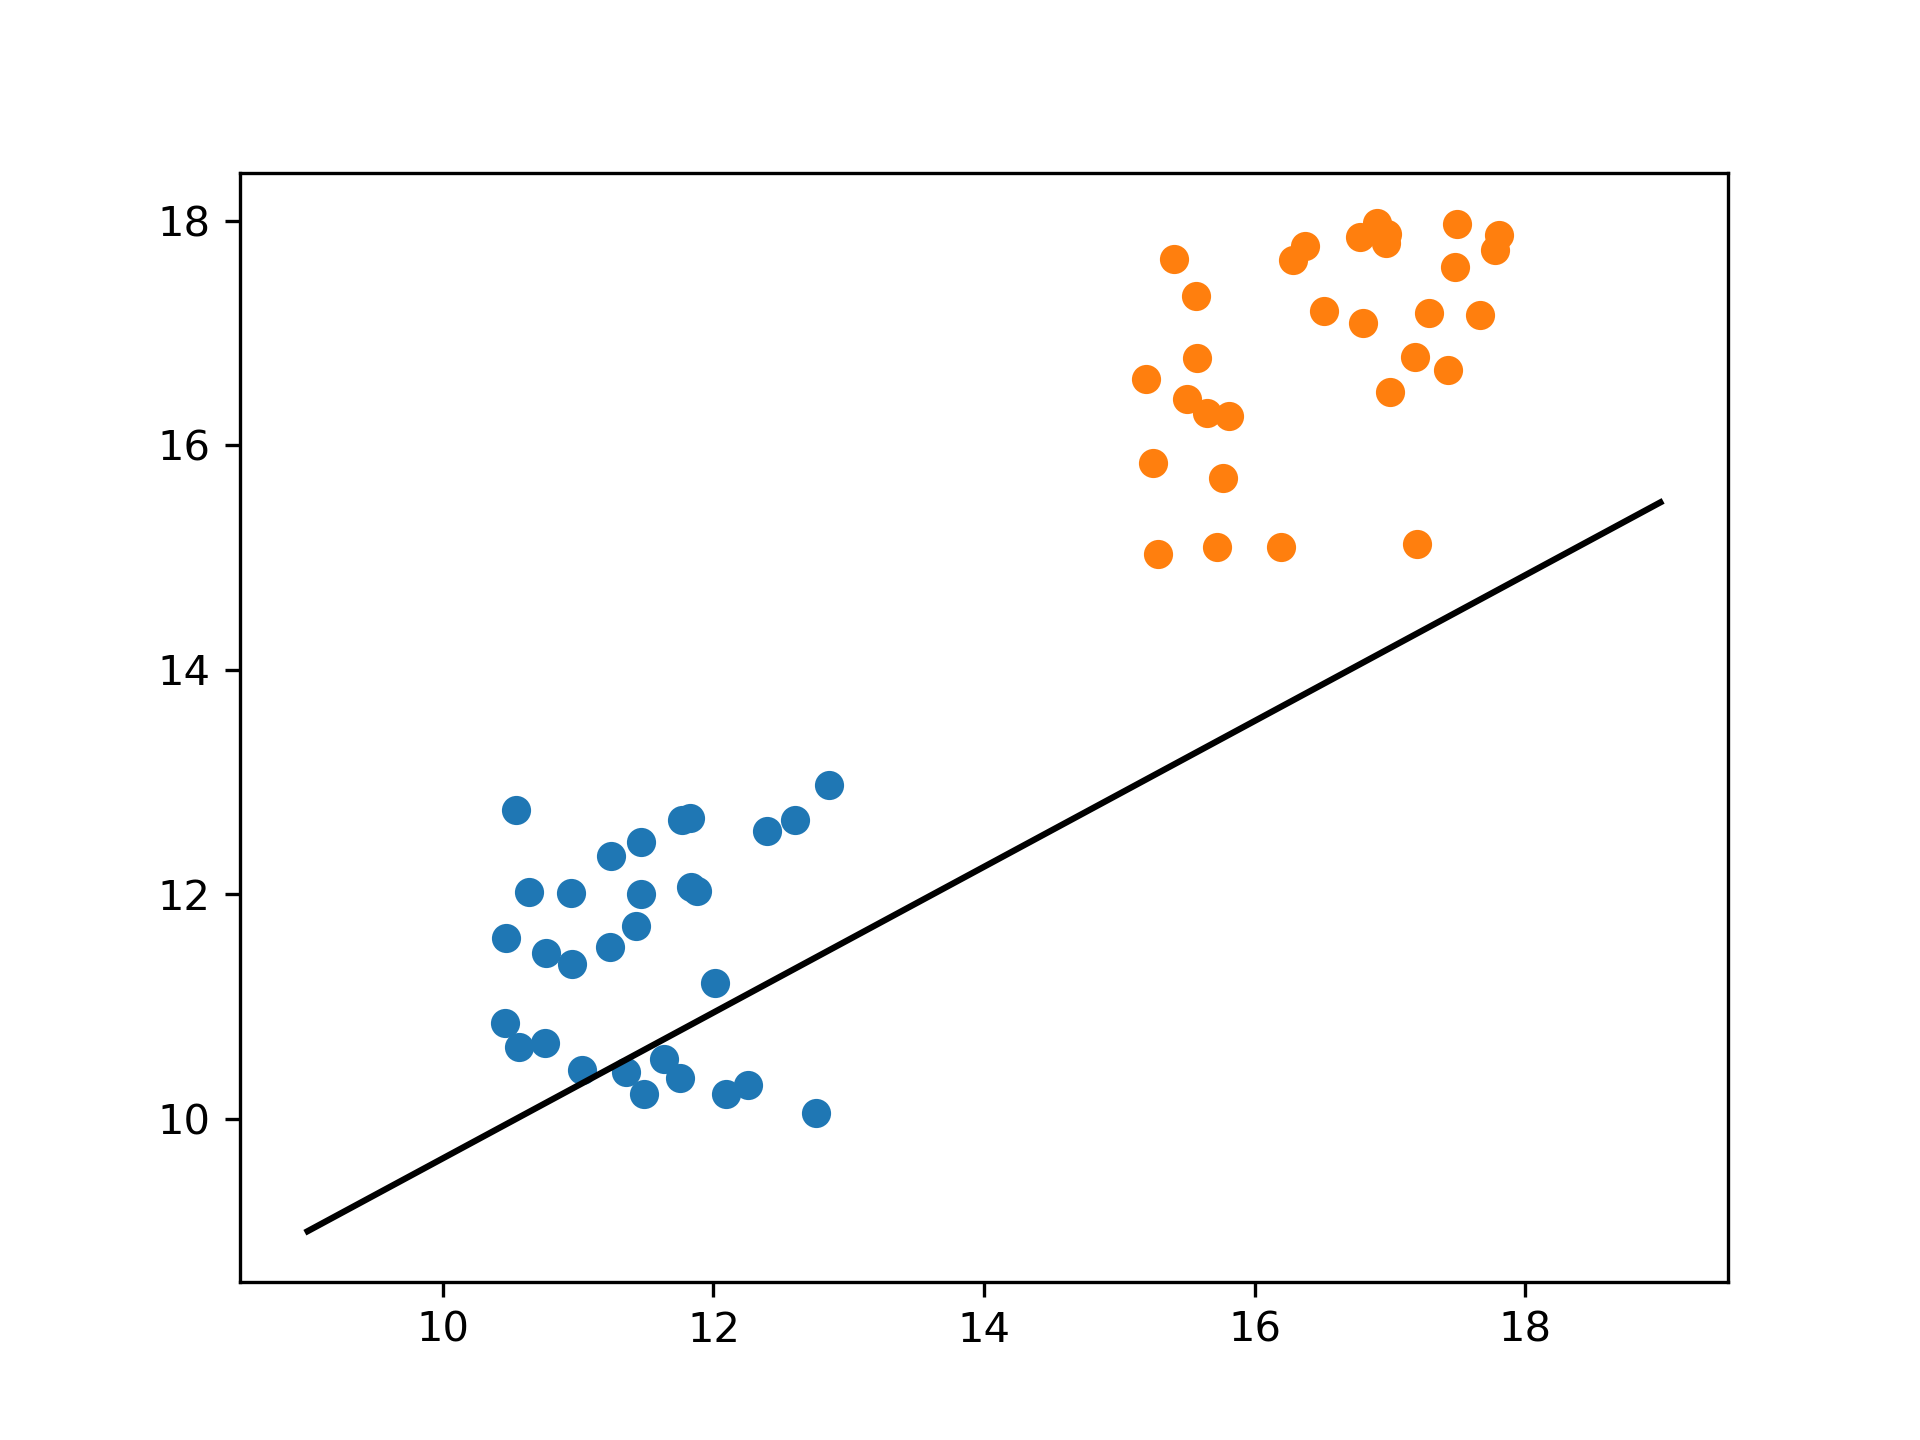
\includegraphics[width = 0.6\textwidth]{Part4/4-3.png}
    \caption{可视化}
\end{figure}

\end{document}


